% 论文数据图内嵌效果演示（references/common.md「T1 期刊规格」指导）：期刊规格 + SciencePlots + Crameri 色图
% 编译：xelatex -interaction=nonstopmode paper_embedded_data.tex（两遍，交叉引用）
% fontset=none：禁止 ctex 自行选择 CJK 字体（它在 Linux 上会去找 Fandol 并可能失败），
% 中英文字体统一由下面的 \input{.../fonts-serif.tex} 决定（见 references/common.md「字体与文字」§1）
\documentclass[12pt,fontset=none]{ctexart}
\ctexset{fontset=none}
\usepackage[a4paper, margin=2.6cm]{geometry}
\usepackage{graphicx}
\usepackage{caption}
\usepackage[subrefformat=parens]{subcaption}
\captionsetup{font=small, labelsep=quad}
\setcounter{section}{2}
\renewcommand{\thefigure}{\thesection.\arabic{figure}}

% ============================================================
% pretty-charts 字体层：衬线搭配（宋体 + Times New Roman）
% 用法：\input{.../references/assets/tikz/fonts-serif.tex}
%
% 为什么单独成文件：示例此前各自写 \setmainfont{Times New Roman}
% + \setCJKmainfont{SimSun}，这两个字体只存在于 Windows，同一份示例在
% Linux/macOS 上无法编译（CI 也就无从编译）。这里按"字体是否存在"逐级回退：
%   Windows  → Times New Roman + SimSun（与原行为完全一致）
%   Linux    → TeX Gyre Termes + Noto Serif CJK SC（apt install fonts-noto-cjk-extra）
%   兜底     → TeX Gyre Termes + FandolSong（TeX Live 自带）
%   再兜底   → 只发警告、不设字体，保证编译不因缺字体而失败（中文可能显示异常）
% \IfFontExistsTF 由 fontspec 提供（preamble.tex 已加载 fontspec）。
% ============================================================
\IfFontExistsTF{Times New Roman}
  {\setmainfont{Times New Roman}}          % Windows / macOS
  {\IfFontExistsTF{TeX Gyre Termes}
     {\setmainfont{TeX Gyre Termes}}        % Linux 需 apt install fonts-texgyre
     {\PackageWarning{pretty-charts}{未找到西文衬线字体（Times New Roman / TeX Gyre %
       Termes），改用 XeLaTeX 默认西文字体；如需一致字形请安装 fonts-texgyre}}}
\IfFontExistsTF{SimSun}
  {\setCJKmainfont{SimSun}}                % 中文宋体（Windows）
  {\IfFontExistsTF{Noto Serif CJK SC}
     {\setCJKmainfont{Noto Serif CJK SC}}   % Linux（fonts-noto-cjk-extra）
     {\IfFontExistsTF{FandolSong}
        {\setCJKmainfont{FandolSong}}        % 兜底：TeX Live 自带，无需系统字体包
        {\PackageWarning{pretty-charts}{未找到中文衬线字体（已尝试 SimSun / %
          Noto Serif CJK SC / FandolSong）；中文可能显示异常。%
          请安装 fonts-noto-cjk-extra，或改用 fonts-sans.tex}}}}


\begin{document}
\section{系统设计与实现}

处理组与对照组的相对表达量在观测期内呈指数分化，处理组第 7 天的表达量约为对照组的
2.1 倍；剂量实验中高剂量组疗效评分显著高于安慰剂组（$p<0.001$），各观测指标间的
相关结构如图~\ref{fig:line}~与图~\ref{fig:panels}~所示。

\begin{figure}[htbp]
  \centering
  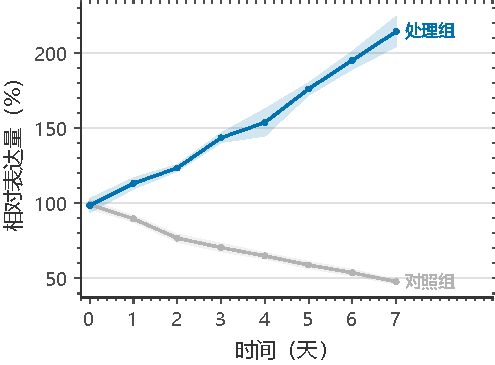
\includegraphics{fig1.pdf}
  \caption{处理组与对照组相对表达量的时间进程。实线为均值，阴影为 95\% 置信带
  （$n=8$ 次/时间点，$t$ 分布）。}
  \label{fig:line}
\end{figure}

图~\ref{fig:line}~按期刊单栏宽度（90\,mm）制作：无图内标题（信息由图注承载）、
线端直接标注系列名、颜色来自 Okabe-Ito 色板并以中性灰标注对照组，缩放后字号
不低于 7\,pt。

\begin{figure}[htbp]
  \centering
  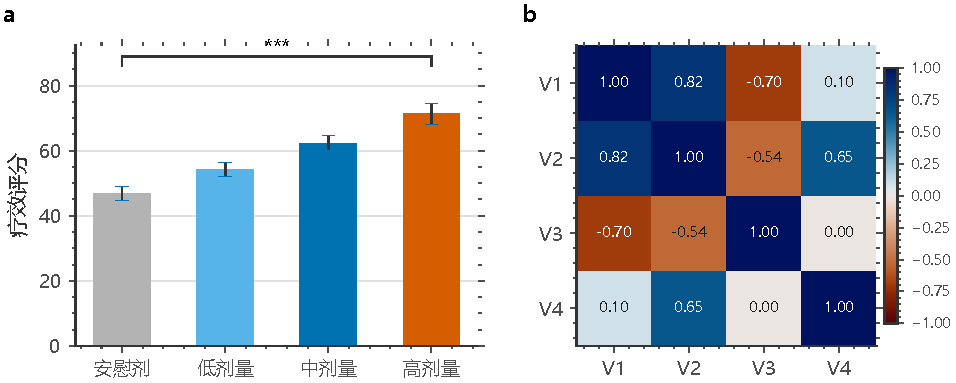
\includegraphics[width=\linewidth]{fig2.pdf}
  \caption{多面板组合示例。(a)~各剂量组疗效评分（均值 $\pm$ 95\%CI，双侧 $t$ 检验，
  $n=32$/组，$***p<0.001$）；(b)~观测指标相关矩阵（Crameri \emph{vik} 发散色图，
  中心对齐零点）。}
  \label{fig:panels}
\end{figure}

图~\ref{fig:panels}~按期刊双栏宽度（190\,mm）制作并拆分为两个面板：面板标签采用
小写粗体字母置于左上角外侧；(a)~中柱状图 y 轴自零点起、误差棒类型在图注中说明；
(b)~采用感知均匀的发散色图并以白色分隔各格。全部图形均为矢量 PDF，字体以内嵌
TrueType 子集形式嵌入，可直接通过出版系统的字体检查。

\end{document}
